\documentclass{article}

\usepackage{caption,color,fancyvrb,subfig}
\usepackage{code,algorithmic,algorithm}
%\usepackage{graphicx,epsfig}
\usepackage{amsmath,amsthm,amsfonts}
%\usepackage{url}
\usepackage{graphicx}
\usepackage{setspace}
\usepackage{bibentry}
 \nobibliography{prelim}

\textwidth = 6.5 in
\textheight = 9 in
\oddsidemargin = 0.0 in
\evensidemargin = 0.0 in
\topmargin = 0.0 in
\headheight = 0.0 in
\headsep = 0.0 in
\parskip = 0.2in
\parindent = 0.0in

\def\inv{^{-1}}


\begin{document}



\begin{titlepage}
\begin{center}

\textsc{\huge \bfseries \sc{Responsive Consistency in Heterogenous,}}\\
\textsc{\huge \bfseries \sc{Wide Area Distributed Storage Systems}}\\[1.0cm]

\emph{A prospectus submitted in partial fulfillment of the degree of Doctor of
Philosophy}\\[5.5cm]

\textsc{\large DRAFT}\\
\emph{October 11, 2016}\\[2.0cm]

\emph{Preliminary Oral Examination for}\\
\textsc{\large Benjamin Bengfort}\\[2.0cm] % [4.0cm]
\emph{Advisor:} \\
\textsc{Dr. Peter J. Keleher}\\[.5cm]
\emph{Committee Members:}\\
\textsc{Dr. Bobby Bhattacharjee}\\
\textsc{Dr. Dave Levin}\\
\textsc{Dr. Neil Spring}\\[4.0cm]

{\bfseries Department of Computer Science}\\
{\bfseries University of Maryland, College Park, MD 20742}\\
{\bfseries December 9, 2016}
\vfill

\end{center}
\end{titlepage}

\newpage
\thispagestyle{empty}
\mbox{}


\newpage
\setcounter{page}{1}
\doublespacing
\begin{abstract}

Data-oriented consistency is not a discrete set of various levels, weak, eventual, causal, strong etc. but rather a continuum that can be adapted in response to environmental conditions. Recent studies of consistency have focused on data center environments which are low latency, high bandwidth, and generally stable; and as a result data distribution involves a relatively small network of devices. I propose to study consistency in a user-oriented context composed of heterogenous devices (mobile phones, desktops, laptops, cloud storage) that can be mobile, creating a network topology of highly variable latency with routine failure and whose networks are larger than typically studied - dozens to hundreds of replica servers.

Our primary context will be a file system that exposes close-to-open consistency and tracks writes to individual objects as a sequence of versions structured as a tree. We consider strong consistency to be a linear sequence of ordered version numbers and inconsistencies to be the presence of forks, misordering, duplicates, or omissions in the version sequence (in order of severity). Additionally we consider the availability of such a system and recognize that enforcement of a linear ordering leads to high latency making the system unusable.

I propose that consistency is primarily related to the network environment as much as it is related to the implemented protocol and as a result, that it can respond the the environment. By creating a system that has a strong central core that maintains a globally consistent view and allowing other replica servers to be flexible I hypothesize that the system will be more consistent than its homogeneous counterparts reducing the number of forks, misordering, duplicates, and omissions as well increasing the throughput and availability of accesses in the system. I propose two primary mechanisms to make this happen:

\begin{enumerate}
    \item \textbf{Federated Consistency}: allow multiple consistency models for different replica servers, integrating over different aspects: temporal, spatial, and synchronization to create a flexible topology of devices with different characteristics and nodes.
    \item \textbf{Hierarchical Consensus}: distribute consensus decisions of sequential ordering in order to make stronger consistency more available.
\end{enumerate}

The experimentation on and development of multi-modal replication protocols via a holistic view will have a large impact in both the data center context as well as in personal distributed file systems.

\end{abstract}
\setstretch{.5}

\newpage
\tableofcontents

\newpage
\listoffigures

\newpage
\doublespacing

%\begin{figure}[!h]
%\begin{center}
%\begin{verbatim}
%/* Sample code snippet */
%\end{verbatim}
%\end{center}
%\caption{Code snippet caption}
%\label{fig:sample_code}
%\end{figure}

% \begin{figure}[!h]
%     \centering
%         \includegraphics[width=.9\textwidth]{figures/figure.png}
%         \caption{Figure caption}
%         \label{fig:label}
% \end{figure}

\section{Introduction}

The rise of virtualized, on-demand computing resources and cloud computing has dramatically shifted the focus of research on consistency in distributed storage systems away from networked file systems toward geographically distributed database management systems, particularly key-value storage. These types of data systems benefit from low-latency, high-bandwidth connections where failure is common due to the magnitude of resources rather than inherent instability. Because most distribution protocols that provide consistency guarantees are dependent on timing parameters related to the latency of messages, it can be shown that consistency is more dependent on network environment than specific protocols. As a result, ``eventually consistent'' \cite{vogels_eventually_2009} systems are said to be consistent enough for most workloads given some probabilistic bounding of staleness \cite{bailis_quantifying_2014,bermbach_eventual_2011,bailis_probabilistically_2012}. This has led consistency research towards investigating stronger forms of eventual consistency, primarily building upon Dynamo \cite{decandia_dynamo:_2007} and Cassandra \cite{lakshman_cassandra:_2010} as reference implementations. Alternatively, research into ensuring strong, sequential consistency in this environment has led to systems like Spanner \cite{corbett_spanner:_2013} which uses atomic and GPS clocks to ensure ``TrueTime'' for sequential ordering or a small number of master nodes that implement consensus algorithms \cite{lamport_paxos_2001,ongaro_search_2014} for locking or ordering \cite{kraska_mdcc:_2013}.

Unfortunately the focus on data center consistency has led to a centralized approach to data storage, forcing a modality where devices must connect to the cloud for file replication even when files exist in the local area \cite{drago_inside_2012}. Although this allows systems to ignore annoyances such as local network configuration and decentralized consistency it does present unnecessary overhead in terms of cost and latency. More pernicious, perhaps, is that users must now buy-in and store their data with a single provider that could go out of business or be hacked leading to research in replicating local data with multiple untrusted cloud stores \cite{zhang_viewbox:_2014,feldman_sporc:_2010}. Finally, there are more devices than ever before connecting to storage applications, partially because users have multiple, heterogenous devices from wearables to workstations and partially because of the advent of the Internet of Things \cite{miorandi_internet_2012}.

We propose to study consistency in user-oriented networks: heterogenous, mobile, variable-latency, and partition-prone topologies with multiple devices and users. Because of the user-centric nature of this research, we further propose the study of a file system as the primary data storage application in such networks. File systems must be highly available such that a user does not notice any delay due to coordination but must also have strong consistency such that any conflicts are presented to the user as soon as possible. To that end, our consistency model must be \textit{responsive} to the network environment providing flexibility when the network is unavailable or laggy and providing strong consistency guarantees when stable connections exist.

Our approach therefore focuses on two primary techniques: the \textit{federation} of weak but available consistency mechanisms with sequential consistency by consensus and the \textit{hierarchical} clustering of quorums so as to minimize conflict by creating localities of interest with global guarantees. We hypothesize that the integration of multi-modal consistency will lead to higher availability than strong consistency models but provide stronger guarantees than eventually consistent systems. We will quantitatively demonstrate the efficacy of such a system by comparing it to homogenous systems with similar sizes and topologies and measuring the number of inconsistencies and amount of latency in both simulation and a real world implementation.

\section{Related Work}

text

\subsection{Consistency}

text

\subsection{Anti-Entropy}

text

\subsection{Consensus}

text

\subsection{Systems}

text

\subsubsection{Bayou}

text

\subsubsection{SUNDR}

text

\subsubsection{Camlistore}

text

\subsubsection{OriFS}

text

\subsubsection{Stellar}

text

\section{Preliminary Work}

We have begun our investigation into the relationship between network environment and consistency by building a discrete event simulator in Python using SimPy that allows us to easily characterize networks and consistency protocols. The simulator has two primary components: workload generators, which act as users that issue read and write accesses to named objects and device processes, which are connected to each other via a specified topology, respond to accesses, generate replication messages, and respond to messages from other devices. Experiments are conducted by running multiple simulations in parallel with different parameters, topological configurations, and accesses. Analysis is conducted on the results of a single simulation or on multiple simulations.

\begin{figure*}
    \centering
    \minipage{0.48\textwidth}
      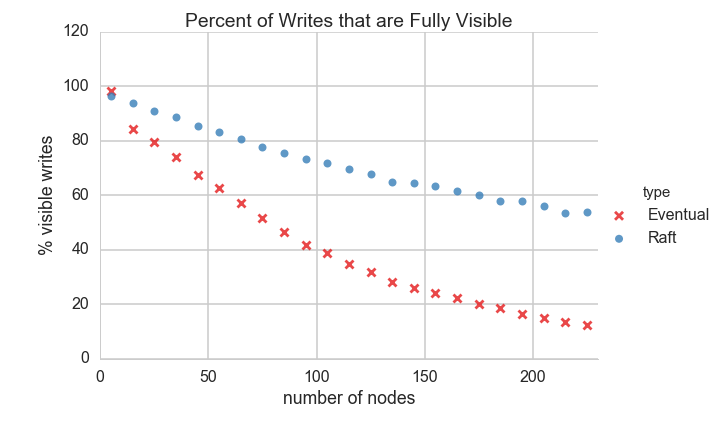
\includegraphics[width=\linewidth]{figures/scaling/visible_writes}
      \caption{Percent of fully visible writes in homogenous eventual and sequential consistency systems.}
      \label{fig:scaling_visible_writes}
    \endminipage\hfill
    \minipage{0.48\textwidth}
      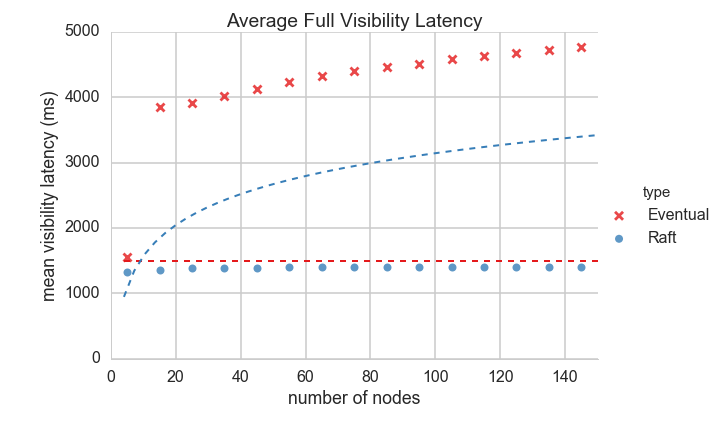
\includegraphics[width=\linewidth]{figures/scaling/visibility_latency}
      \caption{Latency of full visibility in homogenous eventual and sequential consistency systems.}
      \label{fig:scaling_visibility_latency}
    \endminipage
\end{figure*}

Because most research on gossip protocols and quorums specifies small quorums of a size that provide a minimum fault tolerance, our first question related to the effect of consistency protocols with increasing numbers of nodes. We created two homogenous distributed systems: an eventual consistency system implemented with anti-entropy via bilateral gossip and a latest-writer wins policy and sequential consistency by consensus implemented using the Raft consensus algorithm. Each simulation varied the number of nodes in one of five locations, e.g. 5 nodes had one node per location, 25 with 5 nodes per location, up to 100 with 20 nodes per location. Local area latencies were normally distributed with the mean latency, $\lambda_{\mu}=30$ms and the standard deviation of latency, $\lambda_{\sigma}=5$ms whereas wide area latencies were higher and more variable, $\lambda_{\mu}=300$ms and $\lambda_{\sigma}=50$ms.

The timing parameters for both Eventual and Raft are based on the network latency. We first computed a conservative timing parameter, $T=10\lambda_{\mu}$ based on the wide area latency mean. The anti-entropy interval for Eventual consistency is given as $\frac {T} {4} = 750$ms. For Raft, the heartbeat interval is $\frac {T} {2} = 1500$ms and the election timeout is a uniform random selection in the range $U(T, 2T) = U(3000, 6000)$. These conservative timing parameters ensure that it is rare that messages arrive out of order.

As the number of nodes increases, both Raft and Eventual systems start to degrade in terms of the percent of writes that are fully visible as shown in Figure \ref{fig:scaling_visible_writes}. For Eventual, this is because the time to visibility is related to the number of pairwise anti-entropy sessions required to propagate a write to all nodes as shown in Figure \ref{fig:scaling_visibility_latency}, where the blue line represents perfect convergence (not likely given uniform random neighbor selection). Raft on the other hand has a broadcast mechanism related to its heartbeat interval but writes do not become fully visible because they are rejected by the leader as inconsistent.

\begin{figure*}
    \centering
    \minipage{0.48\textwidth}
      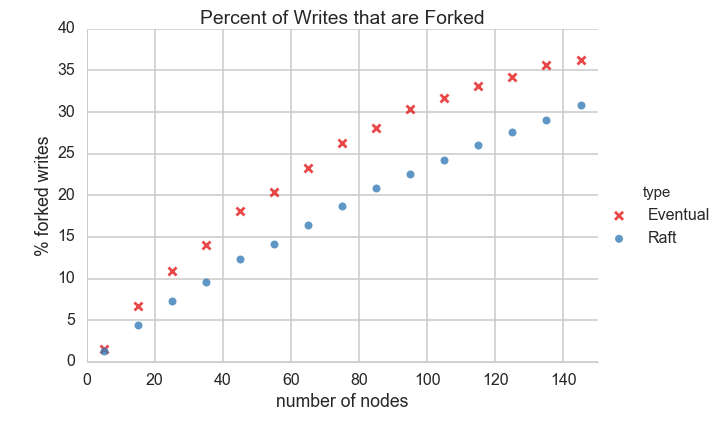
\includegraphics[width=\linewidth]{figures/scaling/forked_writes}
      \caption{Increasing forks in homogenous systems as topology size increases.}
      \label{fig:scaling_forked_writes}
    \endminipage\hfill
    \minipage{0.48\textwidth}
      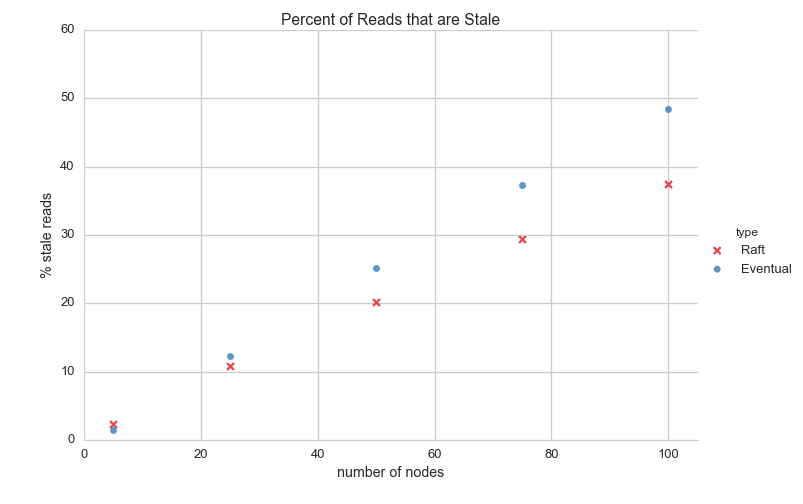
\includegraphics[width=\linewidth]{figures/scaling/stale_reads}
      \caption{Increasing stale reads in homogenous systems as topology size increases.}
      \label{fig:scaling_stale_reads}
    \endminipage
\end{figure*}

Read and write accesses were conducted on each device on 15 objects such that the probability of conflict, $P_c=0.3$ meaning that 30\% of the objects accessed on each device would also be accessed on another device. Accesses were issued at intervals normally distributed with the access interval mean, $A_{\mu}=3000$ms and the access interval standard deviation, $A_{\sigma}=380$ms such that accesses were roughly related to the timing parameter. As the number of nodes increases, the number of conflicts also increase, but not the likelihood of a conflict. Our system measures inconsistencies as \textit{forks} and \textit{stale reads}. As shown in Figure \ref{fig:scaling_forked_writes}, the number of conflicts in Raft is lower than in eventual as are the number of stale reads as shown in \ref{fig:scaling_stale_reads} but at the cost of a performance decrease, particularly as the number of nodes increases.

We believe that these initial investigations show a critical opportunity: that we can blend the high availability of an eventually consistent system and leverage the best parts of anti-entropy and eventual consistency in network environments where messages cannot get through along with the stability and increased visibility of a strongly consistent core, similar to the central core and flexible outer shell proposed by Gray and Oceanstore \cite{gray_dangers_1996,kubiatowicz_oceanstore:_2000}: we call this \textit{Federated Consistency}. Furthermore, if we can find a way to allocate decision space to a smaller number of nodes, we should be able to scale Raft to greater number of nodes without as steep a curve: we investigate this in \textit{Hierarchical Consensus}. Finally, as suggested by the $T$ timing parameter (though not explicitly covered), the timing measures and performance of consistency protocols are related to the network environment, which is dynamic. Potentially we can improve performance by monitoring the environment and adapting timing parameters to minimize the number of inconsistencies: investigated in \textit{Adaptive Consistency}. 

\subsection{Topology}

text

\begin{figure*}
    \centering
    \minipage{0.5\textwidth}
      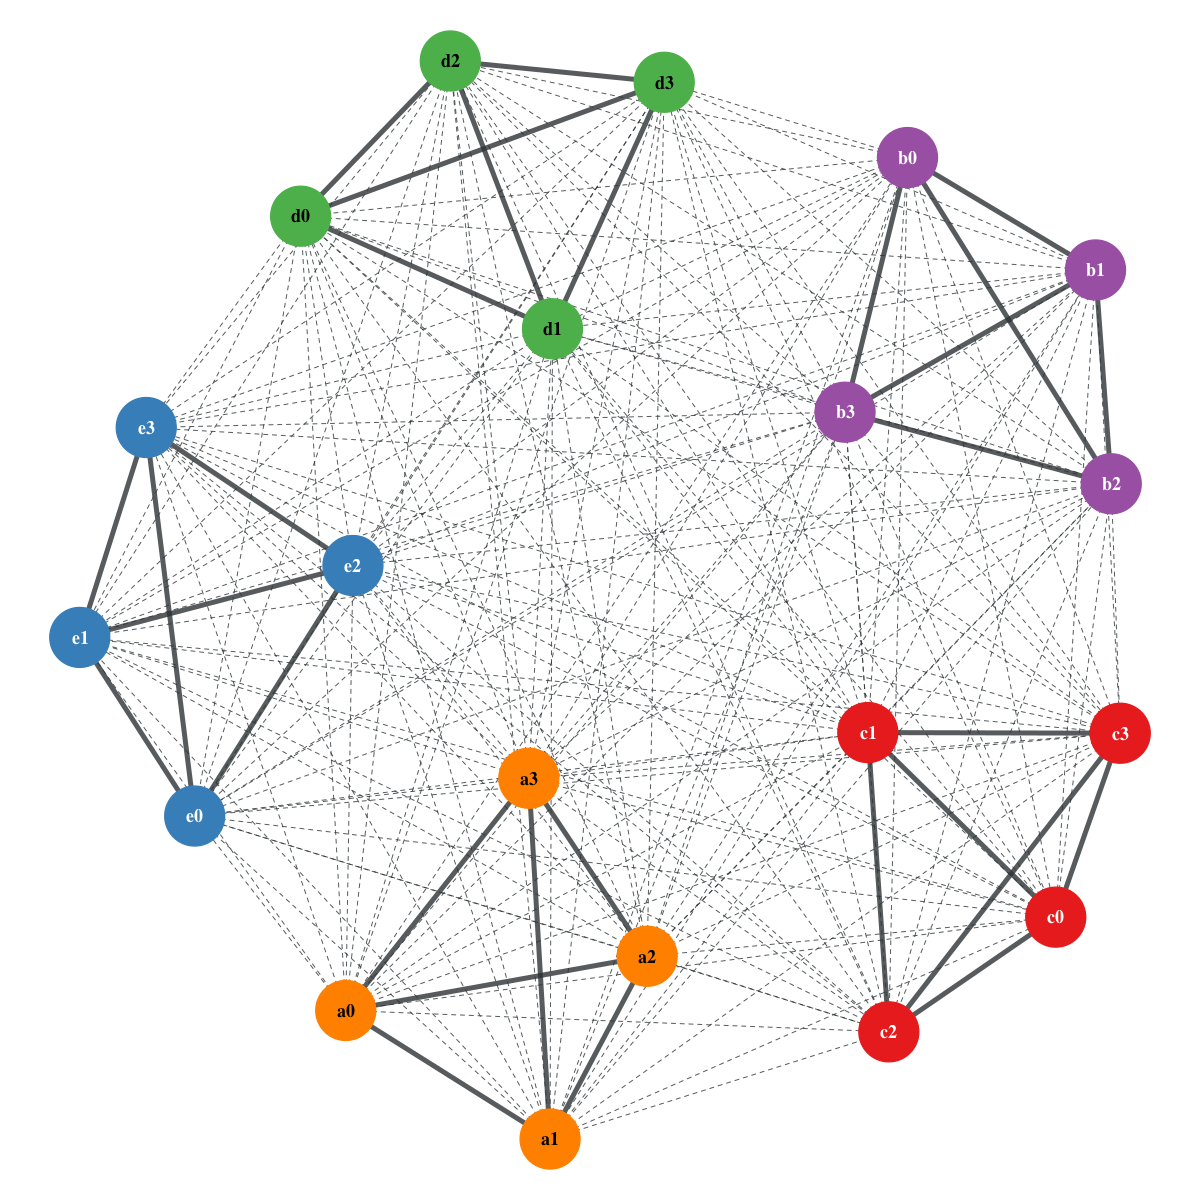
\includegraphics[width=\linewidth]{figures/topology}
      \caption{Proposed Network Topology.}
      \label{fig:topology}
    \endminipage\hfill
    \minipage{0.5\textwidth}
      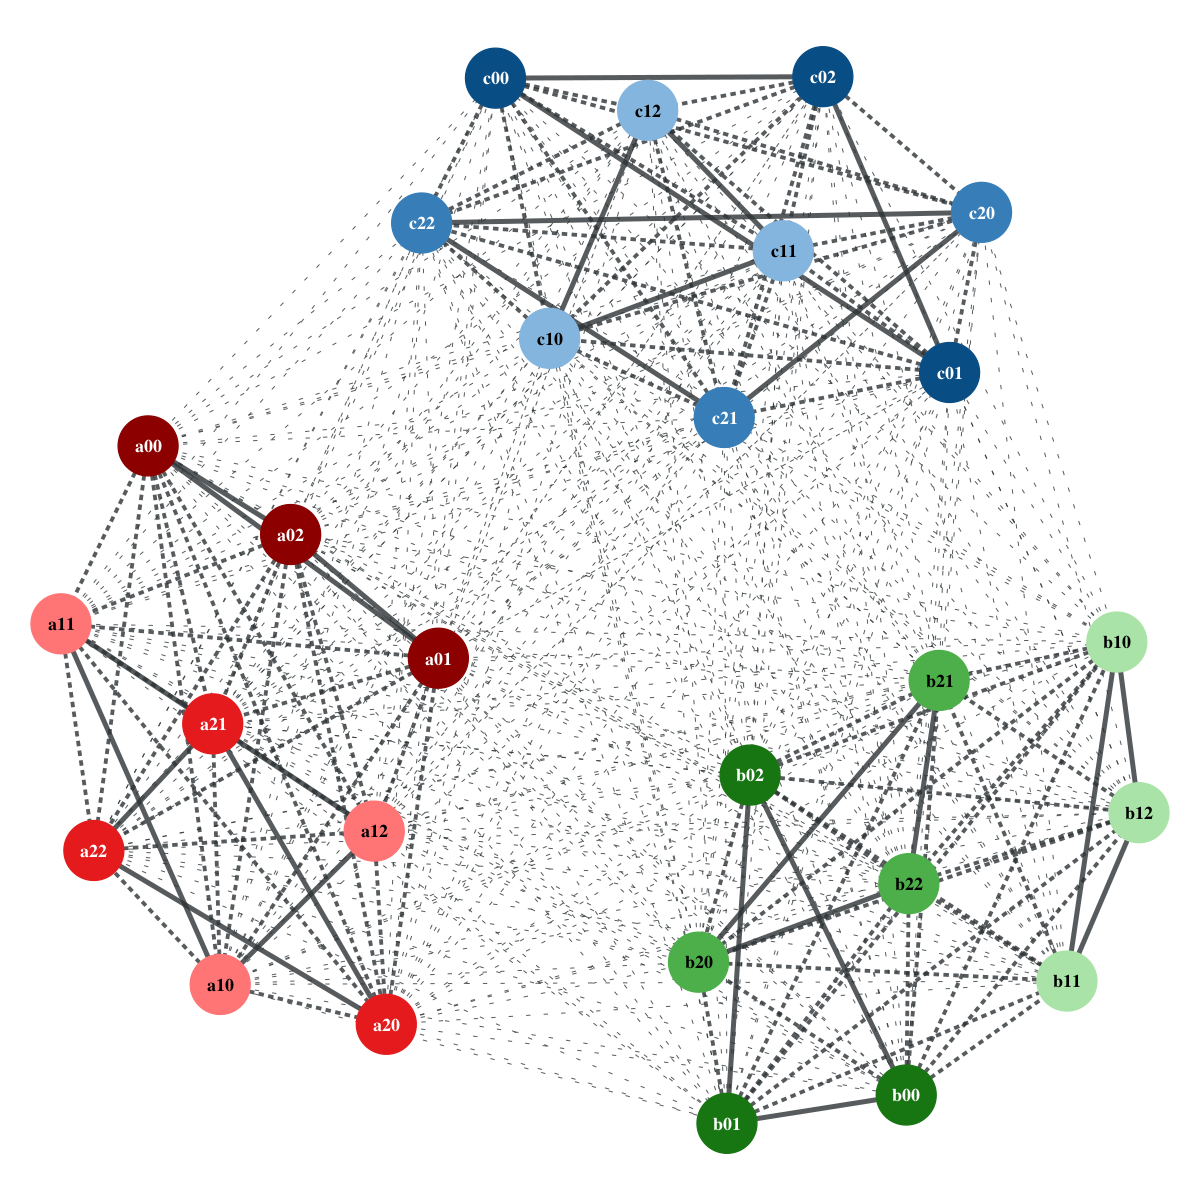
\includegraphics[width=\linewidth]{figures/tiers}
      \caption{Proposed Network Hierarchy.}
      \label{fig:tiers}
    \endminipage
\end{figure*}

\subsection{System Description}

text



text

\section{Proposed Work}

text

\subsection{Federated Consistency}

text

\subsection{Hierarchical Consensus}

text

\subsection{Adaptive Consistency}

text

\section{Timeline}

This is some timeline text.

\begin{center}
\begin{tabular}{|l|c|}
\hline
Federated Consistency & 2 months \\
Hierarchical Consensus & 3 months \\
Flow File System & 4-5 months \\
Adaptive Consistency & 2-3 months \\
\hline
\textbf{TOTAL} & 11-13 months \\
\hline
\end{tabular}
\end{center}

Paper deadline goals:

\begin{itemize}
\item IEEE International Conference on Distributed Computing Systems, June 2017: Federated Consistency
% http://icdcs2017.gatech.edu/
\item ACM Hot Topics in Storage and File Systems 2017, July 2017: Personal Clouds
% https://www.usenix.org/conferences
\item ACM Principles of Distributed Computing, July 2017: Hierarchical Consensus
% http://www.podc.org/
\end{itemize}

text

\section{Conclusion}

Insert conclusion here.

\newpage

\appendix
\section{Appendix A: Reading List}
\label{app:readinglist}

\subsection{Consensus}

1) \bibentry{thomas_majority_1979}

2) \bibentry{lamport_paxos_2001}

3) \bibentry{chandra_paxos_2007}

4) \bibentry{lamport_fast_2006}

5) \bibentry{ongaro_search_2014}


\subsection{Consistency}

1) \bibentry{lamport_time_1978}

2) \bibentry{terry_managing_1995}

3) \bibentry{bailis_quantifying_2014}

4) \bibentry{bailis_potential_2012}

5) \bibentry{bermbach_consistency_2013}


\subsection{Replication}

1) \bibentry{stoica_chord:_2001}

2) \bibentry{kubiatowicz_oceanstore:_2000}

3) \bibentry{gray_dangers_1996}

4) \bibentry{venkataramani_operating_2002}

5) \bibentry{almeida_version_2002}



% \newpage

% \section{Appendix B}
% \label{app:cvtdp2r}


\newpage

\bibliographystyle{plain}
\bibliography{prelim}

\end{document}
